% ===============================
% Data processing
% ===============================
\newpage
\section{Data Processing}
\label{sec:dataproc}

Figure \ref{fig:app_design_perl} shows an overview of the different parts involved in the data importing and analysis process. The \ac{perl} scripts which are reading data from and writing data to the database build the main part of this framework\footnote{The directories in which the scripts, modules and files are located, are listed in table \ref{tab:directories_and_files_overview} on page \pageref{tab:directories_and_files_overview}.}.

\begin{figure}[htpb]
\begin{center}
  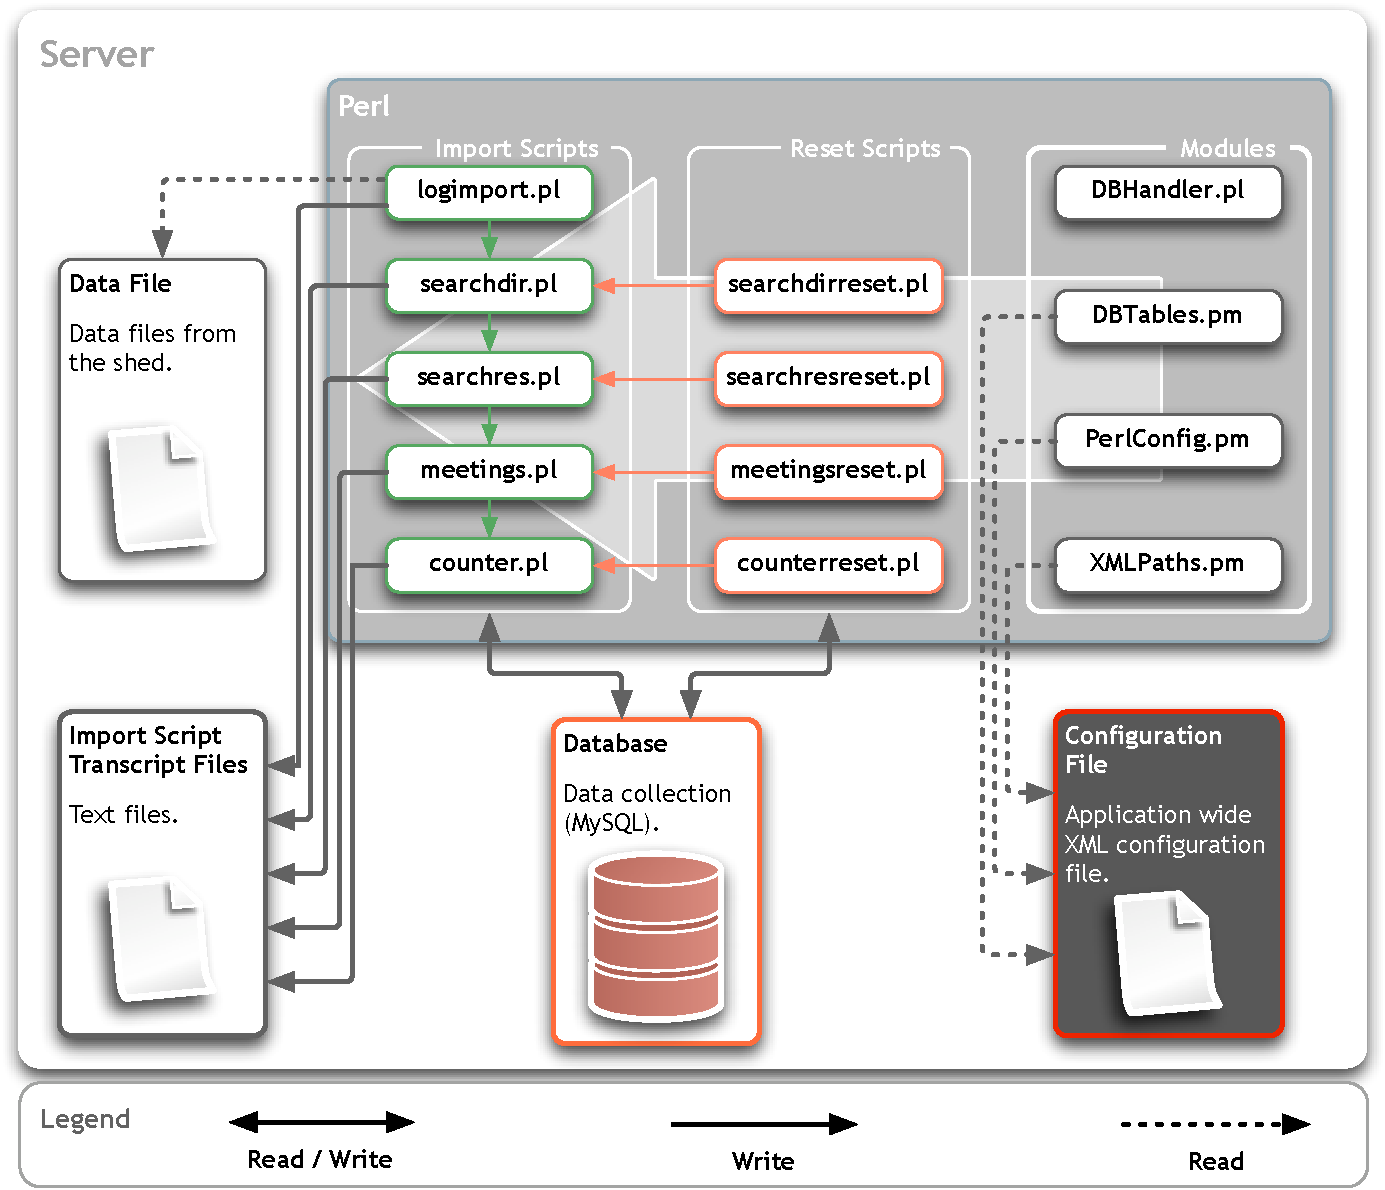
\includegraphics[width=\textwidth]{assets/pdf/app_design_perl.pdf}
  \caption[Data processing overview]{Overview of the parts involved in the data processing.}
  \label{fig:app_design_perl}
\end{center}
\end{figure}

The \textit{Import Scripts} run in a cascade, beginning with the \lstinline|logimport.pl| script, which is reading the data files from the shed, and ending with the \lstinline|counter.pl| script (indicated in figure \ref{fig:app_design_perl} by the green arrows). Each of these scrips writes a transcript file to make their progress traceable. Upon completion of the cascade, the data files are imported and stored in the respective tables as outline in section \ref{subsec:datastorage} on page \pageref{subsec:datastorage}.

A scheduled, daily task checks for new data files uploaded to the server and starts the cascade if needed\footnote{For details about this topic see appendix \ref{app:import_schedule} on page \pageref{app:import_schedule}.}.

The \textit{Reset Scripts} set the database back to a state from where the import cascade can be rerun,  starting with the corresponding import script (indicated in figure \ref{fig:app_design_perl} by the orange arrows). If, for example, the \lstinline|searchdirreset.pl| has been executed, the import cascade can be started with the \lstinline|searchdir.pl| script\footnote{It is recommended to start the import cascade by using the import BASH scripts. This is explained in appendix \ref{app:import_schedule} on page \pageref{app:import_schedule}.}.

The \textit{Modules} read out the configuration and make it available for the import and reset scripts (indicated in figure \ref{fig:app_design_perl} by the large grey arrow with the white border). The whole configuration for the application is stored in an XML file. The part of configuration file accountable for the perl part is shown in appendix \ref{app:configperl} on page \pageref{app:configperl}. As the perl scripts are heavily interacting with the database, the database configuration part of the configuration is read as well by some of the \textit{Modules}\footnote{The database configuration is shown and explained in appendix \ref{app:configdb} on page \pageref{app:configdb}.}. 

\subsection{Importing}
\label{subsec:importing}

The \lstinline|logimport.pl| script writes the data to the \lstinline|data| table as described in section \ref{para:data_table} on page \pageref{para:data_table}.

Prior to the data extraction, the  script creates a backup of the actual database\footnote{The configuration for the backup is explained in appendix \ref{app:configperl} on page \pageref{app:configperl}.}. Subsequently the data is extracted from the data files and written to the database. 

As mentioned in section \ref{subsubsec:problems} on page \pageref{subsubsec:problems}, some of the antennas could not be addressed properly. Therefore, the script has to catch these exceptional values and convert them to the designated ones\footnote{See listing \ref{lst:antenna_adress_conversions} on page \pageref{lst:antenna_adress_conversions} for the detailed conversions.}.  

\subsection{Direction Results}
\label{subsec:dirres}

The \lstinline|searchdir.pl| script searches for matching pairs of antenna readings in the \lstinline|data| table. A pair matches, if 

\begin{mydesc}
\item 

\end{mydesc}

To commit changes made to this value, the \lstinline| searchdirreset.pl| has to be executed followed by the scripts in the import cascade starting with the \lstinline|searchdir.pl| script.    

\subsection{Stay Results}
\label{subsec:stayres}

Aim of the script / step.
Describing code, rules used to calculate the  stay results.

A mouse is termed \textit{nervous}, when she has been read at the inner antenna of the box but not at the outer antenna. The mouse is out of the box only when she is read at the outer antenna of the box.

\subsection{Meeting Results}
\label{subsec:meetingres}

Aim of the script / step.
Describing code, rules used to calculate the association results.